% !TEX TS-program = xelatex
% !TeX program = xelatex
% !TEX encoding = UTF-8
% !TEX spellcheck = fr

%=====================================================================
\ifx\wholebook\relax\else
	\documentclass{KodeBook}
	
\bibliographystyle{unsrtnat}%unsrtnat, plainnat

\hypersetup{
	pdfkeywords={NLP; Language},
	pdfsubject={Artificial intelligence; Natural Language Processing},
	citecolor=blue,
}



\DeclareAcronym{amr}{
	short = AMR,
	long  =  Abstract Meaning Representation,
	tag = abbrev
}

\DeclareAcronym{cfg}{
	short = CFG ,
	long  =  Context Free Grammar,
	tag = abbrev
}

\DeclareAcronym{darpa}{
	short = DARPA ,
	long  = Defense Advanced Research Projects Agency,
	tag = abbrev
}

\DeclareAcronym{edu}{
	short = EDU,
	long  = Elementary Discourse Unit,
	tag = abbrev
}

\DeclareAcronym{fol}{
	short = FOL,
	long  = First Order Logic,
	tag = abbrev
}

\DeclareAcronym{hmm}{
	short = HMM ,
	long  =  Hidden Markov Model,
	tag = abbrev
}

\DeclareAcronym{ia}{
	short = IA ,
	long  = Intelligence Artificielle,
	tag = abbrev
}

\DeclareAcronym{ibm}{
	short = IBM,
	long  = International Business Machines,
	tag = abbrev
}

\DeclareAcronym{idf}{
	short = IDF ,
	long  = Inverse Document Frequency,
	tag = abbrev
}

\DeclareAcronym{ipa}{
	short = IPA ,
	long  = Intelligent Personal Assistant,
	tag = abbrev
}

\DeclareAcronym{iva}{
	short = IVA ,
	long  = Intelligent Virtual Assistant,
	tag = abbrev
}

\DeclareAcronym{ipa2}{
	short = IPA ,
	long  =  International Phonetic Alphabet,
	tag = abbrev
}

\DeclareAcronym{lsa}{
	short = LSA,
	long  = Latent Semantic Analysis,
	tag = abbrev
}

\DeclareAcronym{memm}{
	short = MEMM ,
	long  =  Maximum Entropy Markov Model,
	tag = abbrev
}

\DeclareAcronym{ml}{
	short = ML,
	long  = Machine Learning,
	tag = abbrev
}

\DeclareAcronym{pcfg}{
	short = PCFG ,
	long  = Probabilistic Context Free Grammar,
	tag = abbrev
}

\DeclareAcronym{pdtb}{
	short = PDTB,
	long  = Penn Discourse TreeBank,
	tag = abbrev
}

\DeclareAcronym{ri}{
	short = RI,
	long  =  Recherche d'Information,
	tag = abbrev
}

\DeclareAcronym{rnn}{
	short = RNN ,
	long  = Recurrent Neural Network,
	tag = abbrev
}

\DeclareAcronym{rst}{
	short = RST,
	long  = Rhetorical Structure Theory,
	tag = abbrev
}

\DeclareAcronym{srl}{
	short = SRL,
	long  = Semantic Role Labeling,
	tag = abbrev
}

\DeclareAcronym{svd}{
	short = SVD,
	long  = Singular Value Decomposition,
	tag = abbrev
}


\DeclareAcronym{taln}{
	short = TALN,
	long  = Traitement Automatique du Langage Naturel,
	tag = abbrev
}

\DeclareAcronym{tal}{
	short = TAL ,
	long  = Traitement Automatique des Langues,
	tag = abbrev
}

\DeclareAcronym{tf}{
	short = TF ,
	long  = Term Frequency,
	tag = abbrev
}

\DeclareAcronym{tfidf}{
	short = TF-IDF ,
	long  = Term Frequency - Inverse Document Frequency,
	tag = abbrev
}

\DeclareAcronym{wsd}{
	short = WSD ,
	long  = Word Sense Disambiguation,
	tag = abbrev
}


%\makeglossaries

%\newacronym{oop}{OOP}{Object-oriented programming} 

	\begin{document}
		\mainmatter
	
\fi
%=====================================================================
\changegraphpath{../img/pos/}
\chapter{Étiquetage morpho-syntaxique}

\begin{introduction}[LES \textcolor{white}{L}ANGUES]
	\lettrine{L}{es} catégories grammaticales des mots représentent une caractéristique nécessaire pour comprendre un texte. 
	Des fois, des mots peuvent avoir plusieurs catégories grammaticales (natures). 
	Par exemple, le mot ``nouveau" dans la phrase ``C'est l'anniversaire de mon nouveau[NOM]" n'a pas la même nature que celui dans la phrase ``Mon nouveau[ADJ] cours est presque terminé". 
	Cette propriété peut être aperçue beaucoup plus dans l'anglais où les noms peuvent être transformés en verbes sans changement (Ex. ``fish"). 
	Cette tâche est utile si nous voulons appliquer des statistiques sur les catégories grammaticales afin d'améliorer une autre tâche comme celle de classification des textes. 
	Dans ce chapitre, nous allons présenter la tâche d'étiquetage des séquences en général et l'étiquetage morpho-syntaxique en particulier.
\end{introduction} 

Savoir les catégories grammaticales des mots est un pas vers la compréhension d'une phrase.
Prenons un exemple d'une phrase en anglais : ``\expword{We can can the can}". 
Le mot ``can" a plusieurs sens : (1-verbe) pouvoir (2-verbe) mettre en boîte (3-nom) boîte.
Après étiquetage morpho-syntaxique, nous aurons ``\expword{We[pronom] can[verbe] can[verbe] the[déterminant] can[nom]}".
Ce n'est pas seulement utile pour savoir le sens du mot, mais aussi nous pouvons voir la structure de la phrase.
Essayez d'étiqueter la phrase suivante : ``\expword{Will Will will the will to Will?}".
L'étiquetage morpho-syntaxique est bénéfique pour plusieurs tâches :
\begin{itemize}
	\item c'est une étape préliminaire pour l'analyse syntaxique (chapitre suivant).
	\item les catégories grammaticales peuvent être considérée comme une caractéristique importante dans des tâche de classification des textes. 
	Par exemple, la tâche de détection de l'auteur peut bénéficier de cette caractéristique ; certains auteurs utilisent plus de noms dans les phrases que d'autres.
\end{itemize}


%===================================================================================
\section{Étiquetage de séquences}
%===================================================================================

Un langage peut être considéré comme un phénomène temporel vu que les phrases sont composées d'une séquence continue des mots.
Chaque mot ou ensemble de mots possèdent des caractéristiques linguistiques, chacune définit plusieurs catégories. 
Par exemple, les mots ont des catégories lexicales : nom, verbe, adjectif, etc.
En général, la catégorie d'un mot est dépendante des catégories des mots précédents.
L'étiquetage d'une séquence des mots $w = w_1, \ldots, w_n$ sert à trouver une séquence des étiquettes équivalente $t = t_1, \ldots, t_n$. 

L'étiquetage de séquences peut être réalisé en utilisant des règles définies manuellement. 
Une des méthodes consiste à assigner à chaque mot un ensemble d'étiquettes possibles. 
Ensuite, nous utilisons des règles afin de réduire les étiquettes jusqu'à atteindre une étiquette par mot.
Parmi les règles que nous puissions utiliser : \expword{Un déterminant est suivi par un nom}. 
L'approche statistique vise à apprendre l'annotation en se basant sur un corpus annoté manuellement. 
Le problème de l'étiquetage revient à maximiser la probabilité conditionnelle d'une séquence des étiquettes sachant une séquence des mots (voire l'équation \ref{eq:es-stat}).
\begin{equation}\label{eq:es-stat}
	\hat{t} = \arg\max\limits_t P(t | w)
\end{equation}
Dans les statistiques, il existe deux types de modèles : génératif et discriminatif. 
Un modèle génératif essaye d'apprendre la génération de l'entrée à partir de la sortie ; étant donné une étiquette, quel est la probabilité de chaque mot du vocabulaire ?
En utilisant le théorème de Bayes, l'équation \ref{eq:es-stat} revient à résoudre l'équation \ref{eq:es-stat-gen}.
Le modèle de Markov caché, en anglais \ac{hmm}, est un exemple d'un modèle génératif.
\begin{equation}\label{eq:es-stat-gen}
	\hat{t} = \arg\max\limits_t P(t) P(w | t) 
\end{equation}
Contrairement aux modèles génératifs, un modèle discriminatif estime la probabilité $P(t | w)$ directement. 
Ceci revient à apprendre l'étiquette d'un mot en se basant sur ces caractéristiques en plus des caractéristiques d'un nombre limité des mots avant.
Un modèle qui suit cette méthode est \ac{memm}.
Une autre méthode est d'utiliser les réseaux de neurones récurrents qui supportent l'aspect temporel. 


L'étiquetage morpho-syntaxique est parmi les tâches appartenant à l'étiquetage des séquences. 
Son but est de trouver les catégories grammaticales des mots (nom, verbe, etc.) d'une phrase. 
Des fois, nous voulons détailler les catégories afin d'avoir plus de précision. 
Par exemple, un nom peut être un nom propre ou un nom impropre.
Un exemple d'une phrase en anglais étiquetée morpho-syntaxiquement est illustré dans la figure \ref{fig:ems-exp}.
\begin{figure}[ht]
	\centering
	\hgraphpage[.8\textwidth]{exp-pos2_.pdf}
	\caption[Exemple d'étiquetage morpho-syntaxique.]{Exemple d'étiquetage morpho-syntaxique par \url{https://corenlp.run/} [visité le 2022-05-19].}
	\label{fig:ems-exp}
\end{figure}

Une autre tâche de ce type est la reconnaissance d'entités nommées.
Elle vise à trouver les personnes, les organisations, les places, les nombres, etc. dans une phrase. 
Contrairement à l'étiquetage morpho-syntaxique, une catégorie peut être affectée à une séquence de mots et pas un seul. 
Par exemple, l'expression ``\expword{école nationale supérieure d'informatique}" a la catégorie ``organisation".
Mais, comment exprimer que tous ces mots forment une seule catégorie et pas chaque mot à part ?
La méthode utilisée pour cela est le format \keyword[I]{IOB} (Inside, Outside, Beginning). 
Les mots qui n'appartiennent à aucune catégorie sont annotés par ``O". 
Les mots qui marquent le commencement d'une catégorie sont annotés par ``B-" suivi par le nom de la catégorie. 
Les mots du milieu sont annotés par ``I-" suivi par le nom de la catégorie. 
Donc, l'expression précédente sera annotée comme ``\expword{école[B-ORG] nationale[I-ORG] supérieure[I-ORG] d'informatique[I-ORG]}".
La figure \ref{fig:ner-exp} représente un exemple d'une phrase en anglais contenant des entités nommées.
\begin{figure}[ht]
	\centering
	\hgraphpage[.8\textwidth]{exp-ner2_.pdf}
	\caption[Exemple de la reconnaissance d'entités nommées.]{Exemple de la reconnaissance d'entités nommées par \url{https://corenlp.run/} [visité le 2022-05-19].}
	\label{fig:ner-exp}
\end{figure}

L'analyse syntaxique de surface (Chunking) est un autre exemple d'étiquetage des séquences.
Elle sert à trouver les syntagmes d'une phrase sans structure d'arbre. 
Donc, la catégorie est affectée à une séquence et pas seulement un seule mot.


%===================================================================================
\section{Ressources pour l'étiquetage morpho-syntaxique}
%===================================================================================

Comme mentionné avant, cette tâche sert à trouver la catégorie grammaticale de chaque mot dans une phrase. 
Une catégorie grammaticale peut avoir plusieurs noms (selon l'ouvrage) : nature, catégorie lexicale, classe grammaticale, espèce grammaticale, partie du discours (en anglais, Part of speech).
Afin de réaliser cette tâche, il faut tout d'abord définir les étiquettes (tags). 
Est-ce que nous détaillons les catégories ou nous nous contentons des catégories principales ?
Les étiquettes les plus fameuses sont celles de Penn \keyword[T]{TreeBank} pour l'anglais : conjonction de coordination (CC), nombre cardinal (CD), déterminant (DT), etc. 
Les catégories grammaticales sont différentes d'une langue à une autre. 
Mais, nous pouvons trouver certaines catégories qui sont partagées.
Le projet ``Universal dependencies" cherche à normaliser ces catégories comme indiqué dans le tableau \ref{tab:pos-cat}.

\begin{table}[ht]
	\centering
%	\footnotesize
\begin{tabular}{lll}
	\hline\hline
	\textbf{Classe ouverte} & \textbf{Classe fermée} & \textbf{Autres} \\
	\hline%\hline
	\keyword{ADJ} :  adjectif & \keyword{ADP} : adposition & \keyword{PUNCT} : ponctuation \\
%	\hline
	\keyword{ADV} :  adverbe & \keyword{AUX} : auxiliaire & \keyword{SYM} : symbole \\
%	\hline
	\keyword{INTJ} : interjection & \keyword{CCONJ} : conjonction de coordination & \keyword{X} : Autres \\
%	\hline
	\keyword{NOUN} : nom & \keyword{DET} : déterminant &  \\
%	\hline
	\keyword{PROPN} : nom propre & \keyword{NUM} : numérique &  \\
%	\hline
	\keyword{VERB} : verbe & \keyword{PART} : particule &  \\
%	\hline
	& \keyword{PRON} : pronom &  \\
%	\hline
	& \keyword{SCONJ} : conjonction de subordination &  \\
	\hline\hline
	
\end{tabular}
\caption[Catégories grammaticales universelles]{Catégories grammaticales universelles selon \url{https://universaldependencies.org/u/pos/} [visité le 2021-09-25] \label{tab:pos-cat}}
\end{table}

L'étape suivante est d'annoter un corpus manuellement. 
Ce type de corpus est appelé \keyword[T]{TreeBank}.
Parmi les corpus annotés, nous pouvons citer Penn Treebank pour l'anglais (Exemple dans la figure \ref{fig:penn-exp}).
Un autre projet riche en terme de langues traitées est Universal TreeBank\footnote{Universal TreeBank : \url{https://universaldependencies.org/} [visité le 2021-09-09]} \cite{2012-petrov-al}. 
C'est un projet à communauté ouverte qui vise à utiliser les mêmes classes grammaticales afin d'annoter plusieurs langues. 
Mais, il faut faire attention lorsque nous fusionnons deux treebanks différents. 
Lorsqu'il y a plusieurs tags, nous pouvons trouver des inconsistances dans l'annotation.
Par exemple, dans les corpus ``Brown" et ``WSJ", le mot ``to" a le tag ``TO". 
Dans le corpus ``Switchboard", il a le tag ``TO" lorsqu'il indique l'infinitif, sinon ``IN" lorsque c'est une préposition.

\begin{figure}[ht]
	\centering
	\begin{tcolorbox}[colback=white, colframe=blue, boxrule=1pt, text width=.62\textwidth]
		\footnotesize
		\begin{alltt}
			Battle-tested\keyword{/JJ} Japanese\keyword{/JJ} industrial\keyword{/JJ} managers\keyword{/NNS}
			here\keyword{/RB} always\keyword{/RB} buck\keyword{/VBP} up\keyword{/RP} nervous\keyword{/JJ} newcomers\keyword{/NNS}
			with\keyword{/IN} the\keyword{/DT} tale\keyword{/NN} of\keyword{/IN} the\keyword{/DT} first\keyword{/JJ} of\keyword{/IN}
			their\keyword{/PP\$} countrymen\keyword{/NNS} to\keyword{/TO} visit\keyword{/VB} Mexico\keyword{/NNP} ,\keyword{/,}
			a\keyword{/DT} boatload\keyword{/NN} of\keyword{/IN} samurai\keyword{/FW} warriors\keyword{/NNS} blown\keyword{/VBN}
			ashore\keyword{/RB} 375\keyword{/CD} years\keyword{/NNS} ago\keyword{/RB} .\keyword{/.}
		\end{alltt}
	\end{tcolorbox}
	\caption[Exemple d'un texte annoté de Penn TreeBank.]{Exemple d'un texte annoté de Penn TreeBank ; figure reconstruite de \cite{2003-taylor}.}
	\label{fig:penn-exp}
\end{figure}

Voici quelques applications qui fournissent la tâche d'annotation morpho-syntaxique :
\begin{itemize}
	\item \url{https://nlp.stanford.edu/software/tagger.shtml} [visité le 2021-09-26]
	\item \url{https://github.com/sloria/textblob} [visité le 2021-09-26]
	\item \url{https://www.nltk.org/api/nltk.tag.html} [visité le 2021-09-26]
	\item \url{https://spacy.io/} [visité le 2021-09-26]
	\item \url{https://github.com/clips/pattern} [visité le 2021-09-26]
\end{itemize}

%===================================================================================
\section{Approches d'étiquetage morpho-syntaxique}
%===================================================================================

Ici, nous allons seulement présenter les approches : statistique et neuronale.
Dans l'approche statistique, nous allons présenter le modèle de Markov caché qui  est un modèle génératif, et le modèle de Markov basé sur l'entropie maximale qui est un modèle discriminatif. 
Dans l'approche basée sur les réseaux de neurones, nous allons présenter quelques architectures.

\subsection{Modèle de Markov caché}

Étant donné une séquence des variables d'état $q_1, \ldots, q_i$, l'hypothèse de Markov (comme vu dans le chapitre précédent) affirme que la probabilité d'être dans un état ne dépend que de l'état précédent.
Donc, $ P(q_i | q_1, \ldots, q_{i-1}) \approx P(q_i | q_{i-1}) $.
Une chaîne de Markov peut être formalisée comme un ensemble d'états $Q = \{q_1, q_2, \ldots, q_n\}$, une distribution initiale des probabilités $\pi = [\pi_1, \pi_2, \ldots, \pi_n ],\, \sum_i \pi_i = 1$ et une matrice des  probabilités de transition
$
A = \begin{bmatrix}%
a_{11} & a_{12} & \ldots & a_{1n} \\
a_{21} & a_{22} & \ldots & a_{2n} \\
\vdots & \vdots & \ddots & \vdots \\
a_{n1} & a_{n2} & \ldots & a_{nn} \\
\end{bmatrix}
$

La figure \ref{fig:cm-exp} représente un exemple d'une chaîne de Markov pour la prédiction du temps. 
Il est clair que les états sont $Q = [H, C, W]$ (Hot, Cold, Warm). 
Si nous supposions que la distribution initiale soit $\pi = [0.1, 0.7, 0.2]$, la probabilité de la séquence $H\, W\, C\, C$ serait calculée comme suit :
\begin{align*}
P(H\, W\, C\, C) & = P(H) P(W | H) P(C | H\, W) P(C | H\, W\, C) \\
& = \pi(H) P(W | H) P(C | W) P(C | C) \\
& = 0.1 * 0.3 * 0.1 * 0.8 \\
\end{align*}

\begin{figure}[ht]
	\centering
	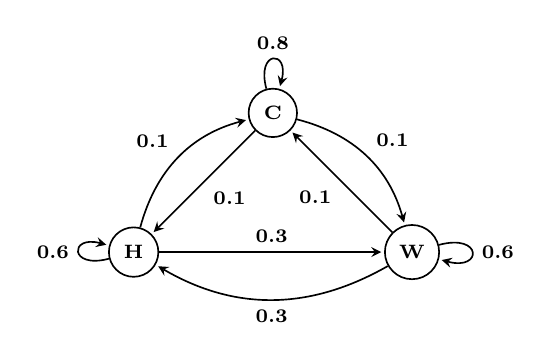
\begin{tikzpicture}[
	> = stealth, % arrow head style
	shorten > = 1pt, % don't touch arrow head to node
	auto,
	node distance = 2.5cm, % distance between nodes
	semithick, % line style
	font=\scriptsize\bfseries
	]
	
	\node[circle,draw] (qC) {C};
	\node[circle,draw] (qH) [below left of=qC] {H};
	\node[circle,draw] (qW) [below right of=qC] {W};
	
	\path[->] 	
	(qC) 	edge [loop above] node {0.8} ()
			edge [] node {0.1} (qH)
			edge [bend left] node {0.1} (qW)
	(qH) 	edge [loop left] node {0.6} ()
			edge [bend left] node {0.1} (qC)
			edge [] node {0.3} (qW)
	(qW)	edge [loop right] node {0.6} ()
			edge [bend left] node {0.3} (qH)
			edge [] node {0.1} (qC);
	\end{tikzpicture}
	\caption[Exemple d'un chaîne de Markov pour la prédiction du temps.]{Exemple d'un chaîne de Markov pour la prédiction du temps ; figure reconstruite de \cite{2019-jurafsky-martin}.}
	\label{fig:cm-exp}
\end{figure}

%\begin{figure}[ht]
%	\centering
%	\hgraphpage[.4\textwidth]{exp-markov_.pdf}
%	\caption[Exemple d'un chaîne de Markov pour la prédiction du temps]{Exemple d'un chaîne de Markov pour la prédiction du temps \cite{2019-jurafsky-martin}\label{fig:cm-exp}}
%\end{figure}

Ceci est un modèle de langage qui ne représente que les probabilités de transition. 
Dans ce cas, nous pouvons seulement représenter la probabilité de transition d'une catégorie à une autre. 
Si nous estimions la probabilité d'émission d'un mot dans chaque état (étiquette), nous pourrions estimer les étiquettes en utilisant la  théorème de Bayes. 
Ce modèle est appelé : modèle de Markov caché (\keyword[H]{\ac{hmm}}) ; les mots d'une séquence sont observés contrairement aux catégories qui sont cachées et doivent être estimées. 
Chaque étiquette (catégorie) $t_i$ est représentée par un un état $q_i$ dans l'ensemble des états $Q = \{q_1, q_2, \ldots, q_n\}$.
Les transitions d'un état vers un autre suivant un modèle Bi-gramme sont représentées par la matrice de transitions $A$.
La distribution initiale des probabilités de ces états est annotée $\pi = [\pi_1, \pi_2, \ldots, \pi_n ]$ où $\sum_i \pi_i = 1$.
Un mot $w_i$ est représenté comme une observation dans la séquences des évènements observés $O = o_1 o_2 \ldots o_T$. 
Une observation $o_t$ peut être générée dans un état $q_i$ avec une probabilités d'observation (probabilités d'émission) $B = b_i(o_t)$.
Un exemple d'un \keyword[H]{\ac{hmm}} est illustré dans la figure \ref{fig:hmm-exp}. 
Les transitions représentent les probabilités de passer d'une étiquette à une autre.
Les missions représentent les probabilités d'occurrence des mots dans les étiquettes.
\begin{figure}[ht]
	\centering
	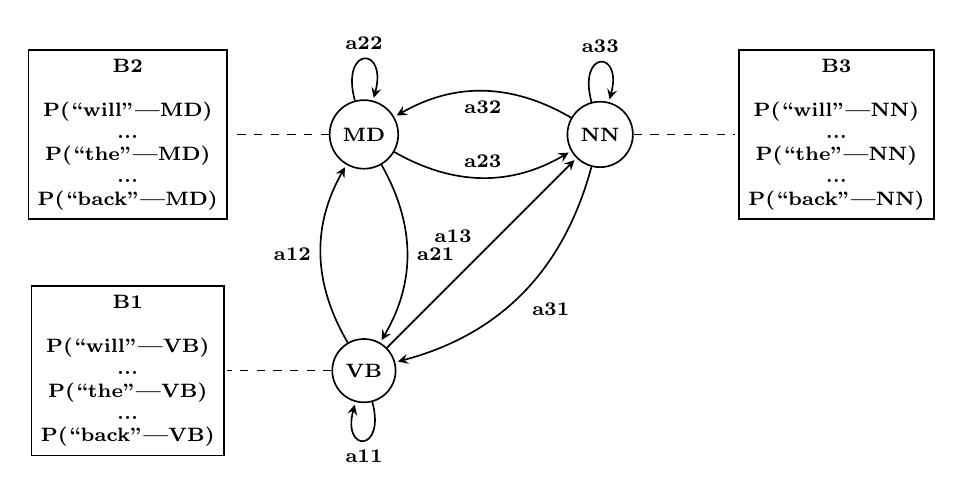
\begin{tikzpicture}[
	> = stealth, % arrow head style
	shorten > = 1pt, % don't touch arrow head to node
	auto,
	node distance = 3cm, % distance between nodes
	semithick, % line style
	font=\scriptsize\bfseries
	]
	
	\node[circle,draw] (q2) {MD};
	\node[align=center,draw] (q2e) [left of=q2] {B2\\ \\P(``will"|MD)\\...\\P(``the"|MD)\\...\\P(``back"|MD)};
	\node[circle,draw] (q3) [right of=q2] {NN};
	\node[align=center,draw] (q3e) [right of=q3] {B3\\ \\P(``will"|NN)\\...\\P(``the"|NN)\\...\\P(``back"|NN)};
	\node[circle,draw] (q1) [below of=q2] {VB};
	\node[align=center,draw] (q1e) [left of=q1] {B1\\ \\P(``will"|VB)\\...\\P(``the"|VB)\\...\\P(``back"|VB)};
	
	\path[->] 	
	(q1) 	edge [loop below] node {a11} ()
			edge [bend left] node {a12} (q2)
			edge [] node {a13} (q3)
	(q2) 	edge [loop above] node {a22} ()
			edge [bend left] node {a21} (q1)
			edge [bend right] node {a23} (q3)
	(q3)	edge [loop above] node {a33} ()
			edge [bend left] node {a31} (q1)
			edge [bend right] node {a32} (q2);
	
	\path[dashed] 	
	(q1) 	edge [] node {} (q1e)
	(q2) 	edge [] node {} (q2e)
	(q3) 	edge [] node {} (q3e);
	
	\end{tikzpicture}
	\caption[Exemple d'une représentation HMM]{Exemple d'une représentation HMM ; figure reconstruite de \cite{2019-jurafsky-martin}.}
	\label{fig:hmm-exp}
\end{figure}

%\begin{figure}[ht]
%	\centering
%	\hgraphpage[.6\textwidth]{exp-hmm_.pdf}
%	\caption[Exemple d'une représentation HMM]{Exemple d'une représentation HMM \cite{2019-jurafsky-martin}\label{fig:hmm-exp}}
%\end{figure}

La séquence estimée $\hat{t}$ est celle qui maximise la probabilité $P(t)$ et la probabilité $P(w | t)$ selon l'équation \ref{eq:hmm-detail}.
En utilisant un modèle \keyword[B]{Bi-gramme}, la probabilité $P(t)$ est calculée en utilisant les transitions de l'état initial $t_1$ jusqu'à le dernier $t_n$. 
Il faut savoir que la probabilité $P(t_1|t_0)$ est en réalité la probabilité initiale $\pi_1$ de l'état $t_1$.
La probabilité $P(w_i | t_i)$ est une probabilité d'émission dans le modèle de Markov caché.
\begin{align}
\hat{t} & = \arg\max\limits_t P(t) P(w | t) \nonumber\\
		& = \arg\max\limits_t P(t_1 \dots t_n) P(w_1 \dots w_n | t_1 \dots t_n) \nonumber\\
		& = \arg\max\limits_t \pi_{t1} \prod_{i=2}^{n} P(t_i|t_{i-1}) \prod_{i=1}^{n} P(w_i| t_i) \nonumber\\
        & = \arg\max\limits_t \prod_{i=1}^{n} \underbrace{P(t_i|t_{i-1})}_{a_{i-1,i}} \underbrace{P(w_i | t_i)}_{b_i(w_i)} \label{eq:hmm-detail}
\end{align}

Avant de discuter comment une séquence $w=w_1 \ldots w_n$ est décodée selon l'équation \ref{eq:hmm-detail}, nous commençons par décrire l'entraînement. 
Dans un \keyword[H]{\ac{hmm}}, les états sont les tags (catégories) $t_i$ et les observations sont les mots $w_i$. 
Notons la fonction qui compte le nombre des occurrence d'une séquence comme $C$.
La probabilité de transition $a_{i-1,i}$ de l'état $t_{i-1}$ vers $t_i$ est estimée à partir du corpus d'entraînement selon l'équation \ref{eq:pos-hmm1}.
Notons ``<s>" ; l'étiquette qui précède la première catégorie de la phrase. 
Dans ce cas, la probabilité $\pi_i$ de commencer par l'état $t_i$ est estimée selon l'équation \ref{eq:pos-hmm2}.
La probabilité d'émission d'un mot $w_i$ dans un état $t_i$ est estimée selon l'équation \ref{eq:pos-hmm3}.
\begin{align}
P(t_i | t_{i-1}) = \frac{C(t_{i-1}, t_i)}{C(t_{i-1})}  \label{eq:pos-hmm1} \\
\pi_i = P(t_i | <s>) = \frac{C(<s>, t_i)}{C(<s>)} \label{eq:pos-hmm2} \\
P(w_i | t_i) = \frac{C(t_i, w_i)}{C(t_i)} \label{eq:pos-hmm3}
\end{align}

Prenons un exemple d'un corpus d'entraînement avec quatre phrases. 
Nous avons 4 catégories : DT, PR, VB et NM. 
\begin{itemize}
	\item un/DT ordinateur/NM peut/VB vous/PR aider/VB
	\item il/PR veut/VB vous/PR aider/VB
	\item il/PR veut/VB un/DT ordinateur/NM
	\item il/PR peut/VB nager/VB  
\end{itemize}
Un exemple de calcul d'une transition est le suivant : $P(VB | NM) = \frac{C(NM,\ VB)}{C(NM)} = \frac{1}{2}$. 
La probabilité d'émission du mot ``veut" lorsque le tag est ``VB" est calculée comme suit : $P(veut | VB) = \frac{C(VB,\ veut)}{C(VB)} = \frac{2}{7}$. 
La probabilité q'un pronom soit au début de la phrase est calculée comme : $\pi_{PR} = \frac{C(<s>,\ PR)}{C(<s>)} = \frac{3}{4} $.
La matrice des transitions ainsi que la distribution initiale sont illustrés dans le tableau \ref{tab:hmm-trans-init}. 
Pourtant ce n'est pas utilisé dans le calcul, nous avons ajouté le passage d'un état vers la fin afin de compléter la distribution (avoir une somme de 1 sur les lignes). 
Les probabilités d'émission sont illustrées dans le tableau \ref{tab:hmm-emission}. 
\begin{table}[ht]
	\centering\footnotesize
\begin{tabular}{llllll}
	\cline{2-6}\noalign{\vskip\doublerulesep
		\vskip-\arrayrulewidth}\cline{2-6}
	     & DT & PR & VB & NM & \textless/s\textgreater\\
	\hline
	DT  &  0  &  0   &  0   &   1  &  0  \\
	PR &  0  &  0   &   1  &  0   &  0  \\
	VB & 1/7 & 2/7  & 1/7  &  0   & 3/7 \\
	NM &  0  &  0   & 1/2  &   0  &  1/2 \\
	\hline
	\textless s\textgreater ($\pi$) &  1/4  &  3/4   & 0  &   0  &  0 \\
	\hline\hline
\end{tabular}
\caption[Exemple des probabilités de transition et une distribution initiale]{Exemple des probabilités de transition et une distribution initiale \label{tab:hmm-trans-init}}
\end{table}

\begin{table}[ht]
	\centering\footnotesize
\begin{tabular}{lllllllll}
	\cline{2-9}\noalign{\vskip\doublerulesep
		\vskip-\arrayrulewidth}\cline{2-9}
	     & un & ordinateur & peut & vous & aider & il & veut & nager \\
	\hline
	DT  &  1 &  0         &  0   &   0  &  0    & 0  & 0    & 0 \\
	PR &  0 &  0         &  0   & 1/4  &  0    &3/4 & 0    & 0 \\
	VB &  0 &  0         & 2/7  &   0  &  2/7  & 0  & 2/7  & 1/7 \\
	NM &  0 &  1         &  0   &   0  &  0    & 0  & 0    & 0 \\
	\hline\hline
\end{tabular}
\caption[Exemple des probabilités d'émission]{Exemple des probabilités d'émission \label{tab:hmm-emission}}
\end{table}

%\begin{figure}
%	\begin{tikzpicture}[
%	> = stealth, % arrow head style
%	shorten > = 1pt, % don't touch arrow head to node
%	auto,
%	node distance = 3cm, % distance between nodes
%	semithick, % line style
%	font=\small
%	]
%	
%	\tikzstyle{every state}=[
%	draw = black,
%	thick,
%	fill = white,
%	minimum size = 4mm
%	]
%	
%	\node[circle,draw] (qN) {N};
%	\node[align=left,draw] (qNe) [left of=qN] {P("fish"|N)=0.05\\P("river"|N)=0.03};
%	\node[circle,draw] (qV) [right of=qN] {V};
%	\node[align=left,draw] (qVe) [right of=qV] {P("fish"|V)=0.01\\P("eat"|V)=0.02};
%	\node[circle,draw] (qD) [below of=qN] {D};
%	\node[align=left,draw] (qDe) [left of=qD] {P("the"|D)=0.3\\P("a"|D)=0.2\\P("an"|D)=0.15};
%	\node[circle,draw] (qP) [right of=qD] {P};
%	\node[align=left,draw] (qPe) [right of=qP] {P("I"|P)=0.2\\P("he"|P)=0.1\\P("she"|P)=0.1};
%	\node[] () [below of=qD, yshift=1.5cm] {$\pi(P, D, V, N) = (0.4, 0.3, 0.1, 0.2)$};
%	
%	
%	\path[->] 	
%	(qN) 	edge [loop above] node {0.3} ()
%	edge [bend left] node {0.7} (qV)
%	(qV) 	edge [loop above] node {0.1} ()
%	edge [bend left] node {0.5} (qN)
%	edge [bend left] node {0.4} (qD)
%	(qD)	edge [bend left] node {1.0} (qN)
%	(qP)	edge [bend right] node {1.0} (qV);
%	
%	\path[dashed] 	
%	(qN) 	edge [] node {} (qNe)
%	(qV) 	edge [] node {} (qVe)
%	(qD) 	edge [] node {} (qDe)
%	(qP) 	edge [] node {} (qPe);
%	
%	\end{tikzpicture}
%	\caption{Exemple}
%\end{figure}

Revenons maintenant au décodage des tags (étiquetage). 
Après l'entraînement d'un modèle de Markov caché $\lambda = (A, B)$, nous voulons l'utiliser pour estimer la séquence des étiquettes $\hat{t} = \hat{t}_1 \hat{t}_2 \ldots \hat{t}_T$ à partir d'une séquence des observations (mots) $w = w_1 w_2 \ldots w_T$ où nous possédons $N$ tags possibles.
Si nous utilisions un décodage par force brute, nous aurions une complexité de $O(N^T)$.
Vu que la maximisation des tags d'une observation (mot) $w_t$ ne dépend que sur les tags de l'observation précédente, nous pouvons résoudre le problème de la recherche en utilisant la programmation dynamique.
Dans chaque étape $t$ de la séquence, nous nous basons sur l'estimation précédente pour calculer les probabilités de tous les tags afin de choisir celui qui maximise la probabilité comme estimation courante. 
Il faut toujours sauvegarder l'état précédent pour revenir en fin d'algorithme. 
Ceci est appelé la recherche \keyword[V]{Viterbi} (voir l'algorithme \ref{algo:viterbi}).
Dans ce cas, la complexité est réduite à $O(N^2T)$ et la recherche reste toujours exacte.

\begin{algorithm}[ht]
	\KwData{$w = w_1 \ldots w_T$, HMM $\lambda = (A, B)$ avec $N$ états}
	\KwResult{$meilleur\_chemin$, $prob\_chemin$}
	
	Créer deux matrices $viterbi[N, T]$ et $backpointer[N, T]$\;
	
	\Pour{état $ s = 1 \ldots N$}{
		$viterbi[s, 1] = \pi_s * b_s(w_1);\, backpointer[s, 1] = 0$ \;
	}
	
	\Pour{$ t = 2 \ldots T$}{
		\Pour{état $ s = 1 \ldots N$}{
			$viterbi[s, t] = \max\limits_{s'=1}^N viterbi[s', t-1] * a_{s',s} * b_s(w_t)$\;
			$backpointer[s, t] = \arg\max\limits_{s'=1}^N viterbi[s', t-1] * a_{s',s} * b_s(w_t)$\;
		}
	}
	
	$prob\_chemin = \max\limits_{s=1}^N viterbi[s, T];\, pointeur\_chemin = \arg\max\limits_{s=1}^N viterbi[s, T]$\;
	
	$meilleur\_chemin$ est le chemin qui commence par $pointeur\_chemin$ et qui suit $backpointer$
	
	\Return $meilleur\_chemin$, $prob\_chemin$\;
	\caption{Algorithme de Viterbi pour encoder une séquence selon un modèle de Markov caché.}
	\label{algo:viterbi}
\end{algorithm}

En utilisant le modèle entraîné dans l'exemple précédent, nous voulons trouver les tags de cette phrase : \expword{il peut aider}. 
Suivant l'algorithme de Viterbi, nous aurons le tableau \ref{tab:hmm-viterbi-exp} où chaque cellule est remplie par les calculs séparés par des points virgules (les états précédent) et le pointeur de retour entre deux crochets. 
Dans la dernière séquence (``aider"), l'état qui maximise la probabilité est ``VB". 
Le retour est l'état 3 (``VB") ayant un retour vers l'état 2 (``PR"). 
Donc, le texte annoté est : \expword{il/PR peut/VB aider/VB}. 

%\begin{table}[ht]
%	\centering\small
%	\begin{tabular}{llll}
%		\cline{2-4}\noalign{\vskip\doublerulesep
%			\vskip-\arrayrulewidth}\cline{2-4}
%		       & il & peut & aider \\
%		\hline
%		\multirow{4}{*}{DET}  &  \multirow{4}{*}{1/4 * 0}& 0 * 0 * 0 & 0 * 0 * 0 \\
%		  &  & 3/4 * 0 * 0 & 0 * 0 * 0\\
%		  &  & 0 * 1/7 * 0 & 6/28 * 1/7 * 0 \\
%		  &  & 0 * 0 * 0 & 0 * 0 * 0\\
%		\multirow{4}{*}{PRON} &  \multirow{4}{*}{3/4 * 1} &  0 * 0 * 0&  0 * 0 * 0\\
%		  &  & 3/4 * 0 * 0 & 0 * 0 * 0\\
%		  &  & 0 * 2/7 * 0 & 6/28 * 2/7 * 0\\
%		  &  & 0 * 0 * 0 & 0 * 0 * 0 \\
%		\multirow{4}{*}{VERB} &  \multirow{4}{*}{0 * 0} & 0 * 0 * 2/7 & 0 * 0 * 2/7 \\
%		  &  & 3/4 * 1 * 2/7 & 0 * 1 * 2/7 \\
%		  &  & 0 * 1/7 * 2/7 & 6/28 * 1/7 * 2/7\\
%		  &  & 0 * 1/2 * 2/7 & 0 * 1/7 * 2/7 \\
%		\multirow{4}{*}{NOUN} &  \multirow{4}{*}{0 * 0} & 0 * 1 * 0 & 0 * 1 * 0 \\
%		  &  & 3/4 * 0 * 0 & 6/28 * 0 * 0 \\
%		  &  & 0 * 0 * 0 & 0 * 0 * 0 \\
%		  &  & 0 * 0 * 0 & 0 * 0 * 0\\
%		\hline\hline
%	\end{tabular}
%	\caption{Un exemple des probabilités d'émission \label{tab:hmm-viterbi-exp}}
%\end{table}

\begin{table}[ht]
	\centering\footnotesize%\scriptsize
	\begin{tabular}{llll}
		\cline{2-4}\noalign{\vskip\doublerulesep
			\vskip-\arrayrulewidth}\cline{2-4}
		& il & peut & aider \\
		\hline
		DT  & $\frac{1}{4} * 0$ [0]& $0 * 0 * 0$; $\frac{3}{4} * 0 * 0$; $0 * \frac{1}{7} * 0$; $0 * 0 * 0$ [2] & $0 * 0 * 0$; $0 * 0 * 0$; $\frac{6}{28} * \frac{1}{7} * 0$; $0 * 0 * 0$ [3]\\
		PR & $\frac{3}{4} * 1$ [0]&  $0 * 0 * 0$; $\frac{3}{4} * 0 * 0$; $0 * \frac{2}{7} * 0$; $0 * 0 * 0$ [2]&  $0 * 0 * 0$; $0 * 0 * 0$; $\frac{6}{28} * \frac{2}{7} * 0$; $0 * 0 * 0$ [3]\\
		VB & $0 * 0$ [0]& $0 * 0 * \frac{2}{7}$; $\frac{3}{4} * 1 * \frac{2}{7}$; $0 * \frac{1}{7} * \frac{2}{7}$; $0 * \frac{1}{2} * \frac{2}{7}$ [2]& $0 * 0 * \frac{2}{7}$; $0 * 1 * \frac{2}{7}$; $\frac{6}{28} * \frac{1}{7} * \frac{2}{7}$; $0 * \frac{1}{7} * \frac{2}{7}$ [3]\\
		NM & $0 * 0$ [0]& $0 * 1 * 0$; $\frac{3}{4} * 0 * 0$; $0 * 0 * 0$; $0 * 0 * 0$ [1]& $0 * 1 * 0$; $\frac{6}{28} * 0 * 0$; $0 * 0 * 0$; $0 * 0 * 0$ [1]\\
		\hline\hline
	\end{tabular}
	\caption[Exemple d'exécution de l'algorithme de Viterbi]{Exemple d'exécution de l'algorithme de Viterbi \label{tab:hmm-viterbi-exp}}
\end{table}


\subsection{Maximum entropy}

Les estimations par \keyword[H]{\ac{hmm}} se basent seulement sur des statistiques des mots. 
Il est difficile d'introduire des caractéristiques comme les suffixes, le majuscule, etc. 
La régression logistique, qui est un modèle discriminatif, peut combiner plusieurs caractéristiques afin d'estimer une probabilité de sortie. 
Malheureusement, cette méthode ne prend pas les séquences en considération.
Nous pouvons utiliser des caractéristiques sur le mot actuel et les mots avant afin d'estimer l'étiquette ; comme dans les \keyword[H]{\ac{hmm}}.
Dans ce cas le modèle sera appelé \acf{memm}.
Le problème revient à maximiser les probabilités individuelles de chaque étiquette $\hat{t}_i$ (voir l'équation \ref{eq:pos-emm-est}). 
\begin{equation}\label{eq:pos-emm-est}
\hat{t} = \arg\max\limits_t P(t | w) = \arg\max\limits_t \prod\limits_{i}  P(t_i | w_i, t_{i-1})
\end{equation}
Notons $s_i^j$ la séquence $s_i \ldots s_j$. 
Afin d'estimer l'étiquette $t_i$ d'un mot $w_i$, nous prenons $l$ mots précédents et $l$ mots suivants, en plus de $k$ tags précédents.
Nous utilisons un ensemble des caractéristiques $f$ où $f_j$ peut être la présence du majuscule dans le mot, etc.
En utilisant la régression logistique, le problème sera formulé comme dans l'équation \ref{eq:memm}.
L'apprentissage vise à minimiser la somme des erreurs d'étiquetage multi-classes de chaque mot (pour chaque mot, nous aurons plusieurs probabilités ; une pour chaque étiquette).
\begin{equation}\label{eq:memm}
\hat{t} = \arg\max\limits_t \prod\limits_{i}  
\frac{exp\left(\sum_j \theta_j f_j(t_i, w_{i-l}^{i+l}, t_{i-k}^{i-1})\right)}%
{\sum_{t' \in tags} exp\left(\sum_j \theta_j f_j(t'_i, w_{i-l}^{i+l}, t_{i-k}^{i-1})\right)}
\end{equation}

Voici une liste des caractéristiques $f$ que nous pouvons utiliser dans cette méthode :
\begin{itemize}
	\item Le mot $w_i$ (en considérant chaque mot comme caractéristique)
	\item Les étiquettes précédentes 
	\item $w_i$ contient un préfixe à partir d'une liste (\textit{len(prefixe)} $\le 4$) 
	\item $w_i$ contient un suffixe à partir d'une liste (\textit{len(suffixe)} $\le 4$) 
	\item $w_i$ contient un nombre 
	\item $w_i$ contient une lettre en majuscule
	\item $w_i$ contient un trait d'union 
	\item $w_i$ est complètement en majuscule
	\item La forme du mot $w_i$ (Ex. \expword{X.X.X}) 
	\item $w_i$ est en majuscule avec un trait et un nombre (Ex. \expword{CFC-12}) 
	\item $w_i$ est en majuscule suivi des mots Co., Inc., etc. dans 3 mots maximum
\end{itemize}

\subsection{Modèle neuronal}

Les réseaux de neurones récurrents sont conçus pour traiter les séquences.
Nous avons vu qu'un \ac{rnn} peut être utilisé comme modèle de langage en passant le mot encodé avec \keyword[O]{One-Hot} en entrée et en estimant le mot suivant sachant le contexte précédent. 
Nous modifions la sortie : à la place des probabilités des mots du vocabulaire, nous essayons d'estimer les probabilités des catégories possibles. 
Nous pouvons, bien sûr, utiliser une couche cachée pour apprendre une représentation plus compacte des mots en entrée (\keyword[E]{embedding}). 
La figure \ref{fig:pos-rnn1} représente un exemple d'un réseau de neurones récurrent pour la détection des étiquettes morpho-syntaxique suivant cette modification.
\begin{figure}[ht]
	\centering
	\hgraphpage[.6\textwidth]{rnn-simple.pdf}
	\caption[RNN simple pour l'étiquetage morpho-syntaxique.]{RNN simple pour l'étiquetage morpho-syntaxique.}
	\label{fig:pos-rnn1}
\end{figure}
%\begin{figure}[!ht]
%	\centering
%	\hgraphpage[.55\textwidth]{rnn-simple_.pdf}
%	\caption[RNN simple pour l'étiquetage morpho-syntaxique]{RNN simple pour l'étiquetage morpho-syntaxique \cite{2019-jurafsky-martin}\label{fig:pos-rnn1}}
%\end{figure}

Si nous voulions avoir des réseaux plus profonds et plus complexes, nous pourrions empiler plusieurs \ac{rnn} ensembles. 
Cela permet au modèle d'apprendre des traitements plus complexes améliorant la prédiction.
Pour entraîner ce modèle, nous aurons besoin d'un grand dataset ; la taille de ce dernier augmente avec le nombre des réseaux empilés.
La figure \ref{fig:pos-rnn2} est une illustration d'un modèle avec deux \ac{rnn} empilés.
\begin{figure}[ht]
	\centering
	\hgraphpage[.7\textwidth]{rnn-stack.pdf}
	\caption[RNNs empilés pour l'étiquetage morpho-syntaxique.]{RNNs empilés pour l'étiquetage morpho-syntaxique.}
	\label{fig:pos-rnn2}
\end{figure}
%\begin{figure}[!ht]
%	\centering
%	\hgraphpage[.55\textwidth]{rnn-stack_.pdf}
%	\caption[RNNs empilés pour l'étiquetage morpho-syntaxique]{RNNs empilés pour l'étiquetage morpho-syntaxique \cite{2019-jurafsky-martin}\label{fig:pos-rnn2}}
%\end{figure}

Dans les modèles neuronaux précédents, l'étiquette courante $t_i$ dépend sur le mot courant $w_i$ et le contexte passé. 
Des fois, savoir le contexte futur peut améliorer la décision courante ; nous pouvons trouver une dépendance entre le mot courant et les mots après. 
Afin d'estimer l'étiquette courante en se basant sur le contexte futur, nous utilisons un \ac{rnn} avec une séquence inversée ; c-à-d. l'étiquette $t_i$ sera dépendante à la séquence $w_n, w_{n-1}, \ldots, w_{i+1}, w_{i}$. 
Afin d'exprimer la bidirectionnalité, nous utilisons deux \ac{rnn} : en avant $RNN_{forward}(w_1^i)$ et en arrière $RNN_{backword}(w_i^n)$. 
Nous calculons la somme entre les deux états cachés $h_i^f \oplus h_i^b$ résultant à un vecteur qui doit passer par une fonction ``softmax" afin d'estimer les probabilités des tags. 
Cette architecture est illustrée dans la figure \ref{fig:pos-rnn3}.
\begin{figure}[ht]
	\centering
	\hgraphpage[.7\textwidth]{rnn-bi.pdf}
	\caption[RNN bidirectionnel pour l'étiquetage morpho-syntaxique.]{RNN bidirectionnel pour l'étiquetage.}
	\label{fig:pos-rnn3}
\end{figure}
%\begin{figure}[!ht]
%	\centering
%	\hgraphpage[.60\textwidth]{rnn-bi_.pdf}
%	\caption[RNN bidirectionnel pour l'étiquetage morpho-syntaxique]{RNN bidirectionnel pour l'étiquetage morpho-syntaxique \cite{2019-jurafsky-martin}\label{fig:pos-rnn3}}
%\end{figure}

Les langues sont toujours en amélioration : ajout des nouveaux mots, des nouvelles formes, etc. 
En plus, nous ne pouvons pas capturer toutes les variations de tous les mots en utilisant un corpus limité surtout dans les langues fortement flexionnelles. 
Afin de représenter les variations morphologiques d'un mot, nous devons descendre au niveau caractère.
Une idée (voir la figure \ref{fig:pos-rnn4}) est d'utiliser un modèle de langage au niveau caractère afin d'encoder un mot et combiner ce code avec le code lexicale (\keyword[O]{One-Hot} ou \keyword[E]{embedding}) du mot. 
Le code résultat sera pris comme l'entrée du réseau récurrent (simple, empilé ou bidirectionnel).
\begin{figure}[ht]
	\centering
	\hgraphpage[0.8\textwidth]{rnn-char.pdf}
	\caption[Embedding de caractères pour l'étiquetage morpho-syntaxique.]{RNN avec des embedding de caractères pour l'étiquetage morpho-syntaxique.}
	\label{fig:pos-rnn4}
\end{figure}
%\begin{figure}[ht]
%	\centering
%	\hgraphpage[0.5\textwidth]{rnn-char1_.pdf}
%	\hgraphpage[0.45\textwidth]{rnn-char2_.pdf}
%	\caption[Embedding de caractères pour l'étiquetage morpho-syntaxique]{RNN avec des embedding de caractères pour l'étiquetage morpho-syntaxique \cite{2019-jurafsky-martin}\label{fig:pos-rnn4}}
%\end{figure}

\sectioni{Discussion}
%\begin{discussion}
Chaque langue doit avoir un mécanisme pour identifier les entités existantes dans le monde (plantes, animaux, villes, etc.) et les actions qu'une entité puisse exécuter (Ex. jouer, lire, exister, etc.). 
Les linguistes font la différence entre la fonction d'un mot dans la phrase en utilisant des catégories. 
Par exemple un nom c'est la référence à un objet (concret ou abstrait), or un adjectif est un mot qui représente une propriété d'un nom. 
Donc, le fait de savoir la catégorie d'un mot aide la compréhension d'une phrase. 
Automatiser la tâche de détection des catégories d'une séquence de mots est une étape vers la compréhension de la phrase. 
Même dans les tâches statistiques (qui n'ont pas besoin de la compréhension), les catégories des mots peuvent être un bon indicateur. 

Étiqueter les mots par leurs catégories grammaticales est une tâche appartenant aux tâches de l'étiquetage des séquences. 
Plusieurs approches ont été utilisées pour résoudre ce problème : par règles, statistique et par réseaux de neurones. 
Les règles sont difficiles à mettre en œuvre ; il faut avoir une connaissance profonde de la langue traitée.
Cette approche a été remplacée par l'approche statistique qui vise à estimer l'étiquette en se basant sur des statistiques sur le mot actuel ainsi que les mots précédents et leurs étiquettes.
Avec l'arrivée des \ac{rnn}, cette tâche a devenue plus facile ; il faut juste avoir un corpus étiqueté avec une taille suffisante. 
Dans les architectures présentées dans ce chapitre, l'entrée d'un \ac{rnn} est une représentation vectorielle du mot courant. 
En réalité, nous pouvons définir des architectures plus complexes en introduisant les caractéristiques d'un mot comme par exemple la présence des suffixes. 
Nous pouvons même encoder tous les suffixes avec l'encodage One-Hot et fusionner ce code avec celui du mot. 

Dans ce chapitre, nous avons présenté l'étiquetage des séquences et plus précisément l'étiquetage morpho-syntaxique. 
Nous avons vu les approches et quelques méthodes utilisées pour résoudre cette tâche. 
Mais la question qui se pose : comment pouvons-nous évaluer un système d'étiquetage des séquences ? 
Tout simplement, cette tâche est un cas spécial de classification : à la place de classer une phrase, nous classons chaque mot (ou partie) à part en tenant compte de leurs interactions (temporelles). 
Donc, les métriques d'évaluation de la classification comme la justesse (accuracy), le rappel (recall), la précision (precision), etc. peuvent être utilisées.
Cela concerne l'évaluation intrinsèque, sinon nous pouvons évaluer l'effet de cette tâche sur une autre (évaluation extrinsèque).
%\end{discussion}

\sectioni{Ressources supplémentaires}
%\begin{ressources}

\subsubsection*{Exercices}

\begin{enumerate}
	\item Voici un modèle de Markov caché pour l'étiquetage morpho-syntaxique : 
	
	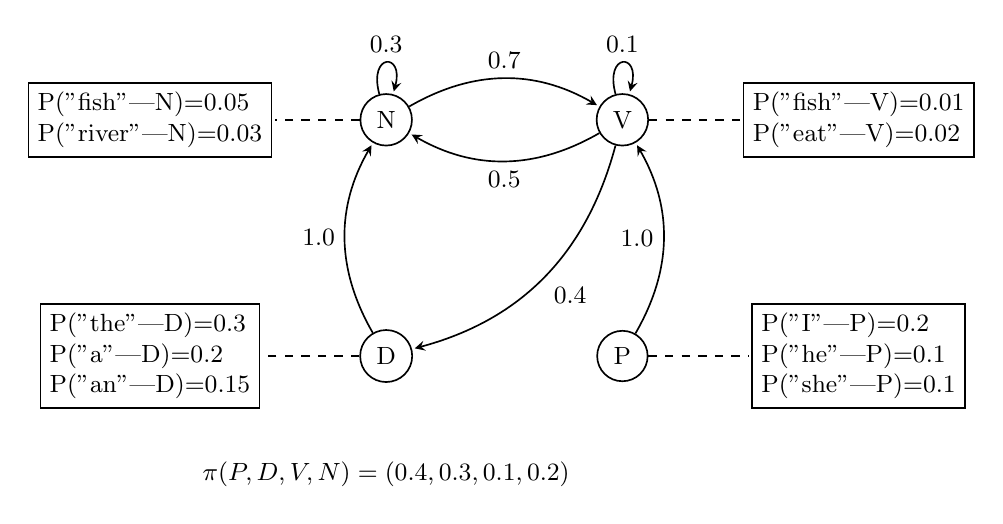
\begin{tikzpicture}[
	> = stealth, % arrow head style
	shorten > = 1pt, % don't touch arrow head to node
	auto,
	node distance = 3cm, % distance between nodes
	semithick, % line style
	font=\small
	]
	
	\tikzstyle{every state}=[
	draw = black,
	thick,
	fill = white,
	minimum size = 4mm
	]
	
	\node[circle,draw] (qN) {N};
	\node[align=left,draw] (qNe) [left of=qN] {P("fish"|N)=0.05\\P("river"|N)=0.03};
	\node[circle,draw] (qV) [right of=qN] {V};
	\node[align=left,draw] (qVe) [right of=qV] {P("fish"|V)=0.01\\P("eat"|V)=0.02};
	\node[circle,draw] (qD) [below of=qN] {D};
	\node[align=left,draw] (qDe) [left of=qD] {P("the"|D)=0.3\\P("a"|D)=0.2\\P("an"|D)=0.15};
	\node[circle,draw] (qP) [right of=qD] {P};
	\node[align=left,draw] (qPe) [right of=qP] {P("I"|P)=0.2\\P("he"|P)=0.1\\P("she"|P)=0.1};
	\node[] () [below of=qD, yshift=1.5cm] {$\pi(P, D, V, N) = (0.4, 0.3, 0.1, 0.2)$};
	
	
	\path[->] 	
	(qN) 	edge [loop above] node {0.3} ()
	edge [bend left] node {0.7} (qV)
	(qV) 	edge [loop above] node {0.1} ()
	edge [bend left] node {0.5} (qN)
	edge [bend left] node {0.4} (qD)
	(qD)	edge [bend left] node {1.0} (qN)
	(qP)	edge [bend right] node {1.0} (qV);
	
	\path[dashed] 	
	(qN) 	edge [] node {} (qNe)
	(qV) 	edge [] node {} (qVe)
	(qD) 	edge [] node {} (qDe)
	(qP) 	edge [] node {} (qPe);
	
	\end{tikzpicture}
	
	\begin{enumerate}
		\item Calculer les deux probabilités : P(V D N | ``fish a fish") et P(N D N | "fish a fish")
		\item Étant donné que C(N) = 200, C(V) = 100 et C(D)=100, calculer les probabilités suivantes en utilisant le lissage de Laplace : P(D|V), P(D|N) et P(N|D).
		\item Recalculer les probabilités de la première question après le lissage.
		\item Combien d'expressions étiquetées ``\textbf{V D N}" existent-elles dans notre dataset d'entraînement ? Le déterminant ``\textbf{D}" ne se produit jamais à la fin de la phrase. 
		
	\end{enumerate}
	
\end{enumerate}

\subsubsection*{Tutoriels}

Les tutoriels sont accessibles via le répertoire Github.
Dans le premier tutoriel, nous présentons la tâche d'étiquetage morpho-syntaxique avec NLTK qui est un outil implémenté en python destiné pour TALN.
Plusieurs algorithmes sont utilisés : RegEx, CRF, HMM, Perceptron et Brill.
Nous présentons, aussi, la tâche d'extraction des entités nommées et celle d'extraction des syntagmes nominaux.

Le deuxième tutoriel utilise flair ; un outil en python pour TALN.
Nous présentons les deux tâches : étiquetage morphosyntaxique et extraction des entités nommées.
Dans le tutoriel, nous pouvons apprendre comment utiliser un modèle existant et comment créer un nouveau modèle.

\subsubsection*{TP : Analyse morphosyntaxique}

On veut concevoir un petit programme pour l'analyse morphosyntaxique à partir de zéro. 
Le modèle HMM avec lissage de Laplace est fourni.
L'étudiant doit implémenter la méthode de décodage ``viterbi".

L'énoncé complet du TP ainsi que les codes et les données sont téléchargeables à partir du répertoire Github.
Le TP est implémenté complètement à partir de zéro (from scratch) : le module HMM et le module qui l'utilise pour l'analyse morphosyntaxique. 
L'étudiant doit compléter deux fonctions du premier module : notation ($p(t_i|t_{i-1}, w_i)$) et décodage viterbi.
Deux autres algorithmes de décodage sont implémentés : force brute et gourmand.
L'étudiant doit comparer entre les trois modèles en calculant la complexité en temps.
Les langages de programmation disponibles (pour l'instant) sont : Java, Javascript/nodejs et Python.

%\subsubsection*{Lab}
%
%Dans la tâche du "Jugements d'acceptabilité", on essaye de deviner si une phrase est acceptable grammaticalement. 
%Par exemple, l'expression "\textbf{Le livre qu'ont puisse trouvé sur internet ...}" ne peut pas être considérée comme acceptable. 
%La raison est que le verbe "ont (avoir)" est moins probable de suivre "que" et que le verbe "puisse (pouvoir)" est conjugué en présent subjonctif, or il est plus probable d'être en infinitif s'il suit le verbe "avoir".
%Dans ce lab, on va essayé de tester des différents modèles de langages afin d'accomplir cette tâche.
%
%L'énoncé complet du lab est téléchargeable à partir du répertoire Github.
%Les outils utilisés sont NLTK et Keras.

%=====================================================================
\ifx\wholebook\relax\else
% \cleardoublepage
% \bibliographystyle{../use/ESIbib}
% \bibliography{../bib/RATstat}
	\end{document}
\fi
%=====================================================================
